\section{Grover's Algorithm}
\label{part1}

Grover's algorithm is a quantum search algorithm that allows searching for an element among $N$ unsorted items in $\mathcal{O}(\sqrt{N})$ time.
Under the same conditions, a classical search algorithm, even a probabilistic one, cannot do better than a search in $\mathcal{O}(N)$ time. \cite{grover1996fast}.
 

\subsection{Description}

More formally, let $N \in \mathbb{N}, \ \omega \in [\![0, N-1]\!]$ and $f = \mathbbm{1}_{\{ \omega \}}$ be the indicator function of the \textit{solution} $\omega$.
Grover's algorithm consists of finding $\omega$ in the set $[\![0, N-1]\!]$ using only a number of calls to the function $f$ proportional to $\sqrt{N}$. 
\\
To do this, we represent the elements of $[\![0, N-1]\!]$ in $\mathcal{H} = (\mathbb{C}^2)^{\otimes n}$, a Hilbert space of dimension $2^n$, which can be implemented by a quantum register using $n=\lceil{\log_{2} N} \rceil$ qubits.\footnote{Note that if $N$ is not a power of 2, some dimensions (and consequently, some qubits) of $\mathcal{H}$ are not used. }
\\
More precisely, this involves the isomorphism:
\begin{align*}
	\Phi : [\![0, N-1]\!] &\longrightarrow \mathcal{H} \\
	x &\longmapsto | x \rangle = | \mathscr{B}(x, n)\rangle
\end{align*}
Where $\mathscr{B}(x, n)$ is the base-2 representation of $x$ encoded on $n$ bits.\footnotemark
\footnotetext{For $x=3$ and $N=7$ for example, we have $\Phi(2) = |010\rangle = |0\rangle \otimes |1\rangle \otimes |0\rangle \in (\mathbb{C}^2)^{\otimes 3}$ }
\\
Note that the states $| x \rangle$ form an orthonormal basis of $\mathcal{H}$, indeed they are the components of the canonical basis of $(\mathbb{C}^2)^{\otimes n}$.
We then define the unitary operator $U_{\omega}$ (called oracle) such that $U_{\omega}|x\rangle = (-1)^{f(x)}|x\rangle$. 
\\
The algorithm thus returns $\omega$ with a probability greater than 1/2 using $\mathcal{O}(\sqrt{N})$ calls to $U_{\omega}$. Furthermore, this probability converges to 1 by increasing the number of executions.

\subsection{Algorithm}
Let $r\in \mathbb{N}$ be the integer closest to $\frac{\pi}{4} \sqrt{N}$.
\begin{itemize}
	\item[1] Initialize the system to the uniform superposition of all states:
	\begin{align}
	|\psi \rangle = |\psi_{(0)}\rangle = \frac{1}{\sqrt{N}} \sum_{k=0}^{N-1} |k\rangle
    \label{init}
	\end{align}
	\item[2] Apply Grover's iteration $r$ times:
	\item[] For $i \in [\![0, r-1]\!]$,
	\begin{itemize}
   	 
    	\item[2.1] Apply the oracle $U_{\omega}$ to $|\psi_{(i)}\rangle$, also given by the formula:
    	\begin{align}
    	U_{\omega} = Id -  2|\omega \rangle \langle \omega |
    	\label{Uomega}
    	\end{align}
    	\item[2.2] Apply Grover's diffusion operator $U_{\psi}$ to $|\psi_{(i)}\rangle$:
    	\begin{align}
    	U_{\psi} = 2|\psi\rangle \langle \psi | - Id
        \label{Upsi}
    	\end{align}
	\end{itemize}
	\item[] Thus we obtain $|\psi_{(i+1)}\rangle = U_{\psi}U_{\omega} |\psi_{(i)} \rangle$. 
	\item[3] Measure the resulting state $|\psi_{(r)} \rangle$.
\end{itemize}

\noindent Morally, the algorithm consists of performing a series of rotations on the state $|\psi \rangle$ so that it gets as close as possible to the state $|\omega \rangle$ in the vector space $\mathcal{H}$, as illustrated by Figure \ref{fig:grover}. 
This allows, upon measuring the resulting state, obtaining the desired state with high probability. 
We observe that at each iteration, the algorithm amplifies the amplitude\footnotemark \, of the vector $|\omega\rangle$ superposed in the vector $|\psi\rangle$. This amplification gives the name to Grover's algorithm's generalizing technique and also provides us with illustration \ref{fig2:subfigures} presented in the appendix.

\footnotetext{For a state vector $|\psi\rangle$ decomposed as a linear combination (superposition) of vectors: $|\psi\rangle = \sum_i \alpha_i |\psi_i\rangle$, the complex numbers $\alpha_i$ are called amplitudes. The probability of obtaining a vector $|\psi_i\rangle$ upon measurement is given by $|\alpha_i|^2$, which gives us $\sum_i |\alpha_i|^2 = 1$. }

\subsection{Proof of Validity}

The algorithm begins with $|\psi \rangle \in F = \mathrm{Vect}(|\psi \rangle , |\omega \rangle )$. 
\\
By the Gram-Schmidt orthonormalization process, we have $(|\psi' \rangle, | \omega \rangle)$ as an orthonormal basis of $F$ with 
\[|\psi'\rangle = \frac{1}{\sqrt{N-1}}\sum_{x \neq \omega} |x \rangle\]
the orthogonal projection of $|\psi \rangle$ onto $\mathrm{Vect}(|\omega \rangle )^{\perp}$, normalized. 
\\
The operator $U_{\omega}$ is an orthogonal symmetry with respect to the hyperplane $\mathrm{Vect}(|\omega \rangle)^{\perp}$, which explains the formula given by \eqref{Uomega}. It is therefore in particular a symmetry with respect to $|\psi'\rangle$ for the elements of $F$.
The operator $U_{\psi}$ given by \eqref{Upsi} is an orthogonal symmetry with respect to $|\psi\rangle$.
We also note that $F$ is stable by $U_{\omega}$ and $U_{\psi}$, thus the states $|\psi_{(i)} \rangle$ remain in the vector subspace $F$ during the entire execution of the algorithm.
\\
At each iteration, the operator $Q=U_{\psi} U_{\omega}$ performs a rotation by $2\theta$ with:
\[\theta = \mathrm{arcsin}(\frac{1}{\sqrt{N}})\]
Thus with enough rotations, we can orient the initial state towards $|\omega \rangle$.
However, it is crucial to stop the algorithm when the state vector approaches $|\omega \rangle$, because if the targeted state is surpassed, subsequent rotations will move $|\psi_{(i)} \rangle$ away from $|\omega \rangle$.
The exact measurement probability is given by:
\[\mathrm{sin}^2 \left( \left( 2r + 1 \right) \theta \right) \]
We will explain this value later. 
\begin{figure}
\hspace{1.2cm}
\begin{adjustbox}{minipage=1.2\textwidth, right}
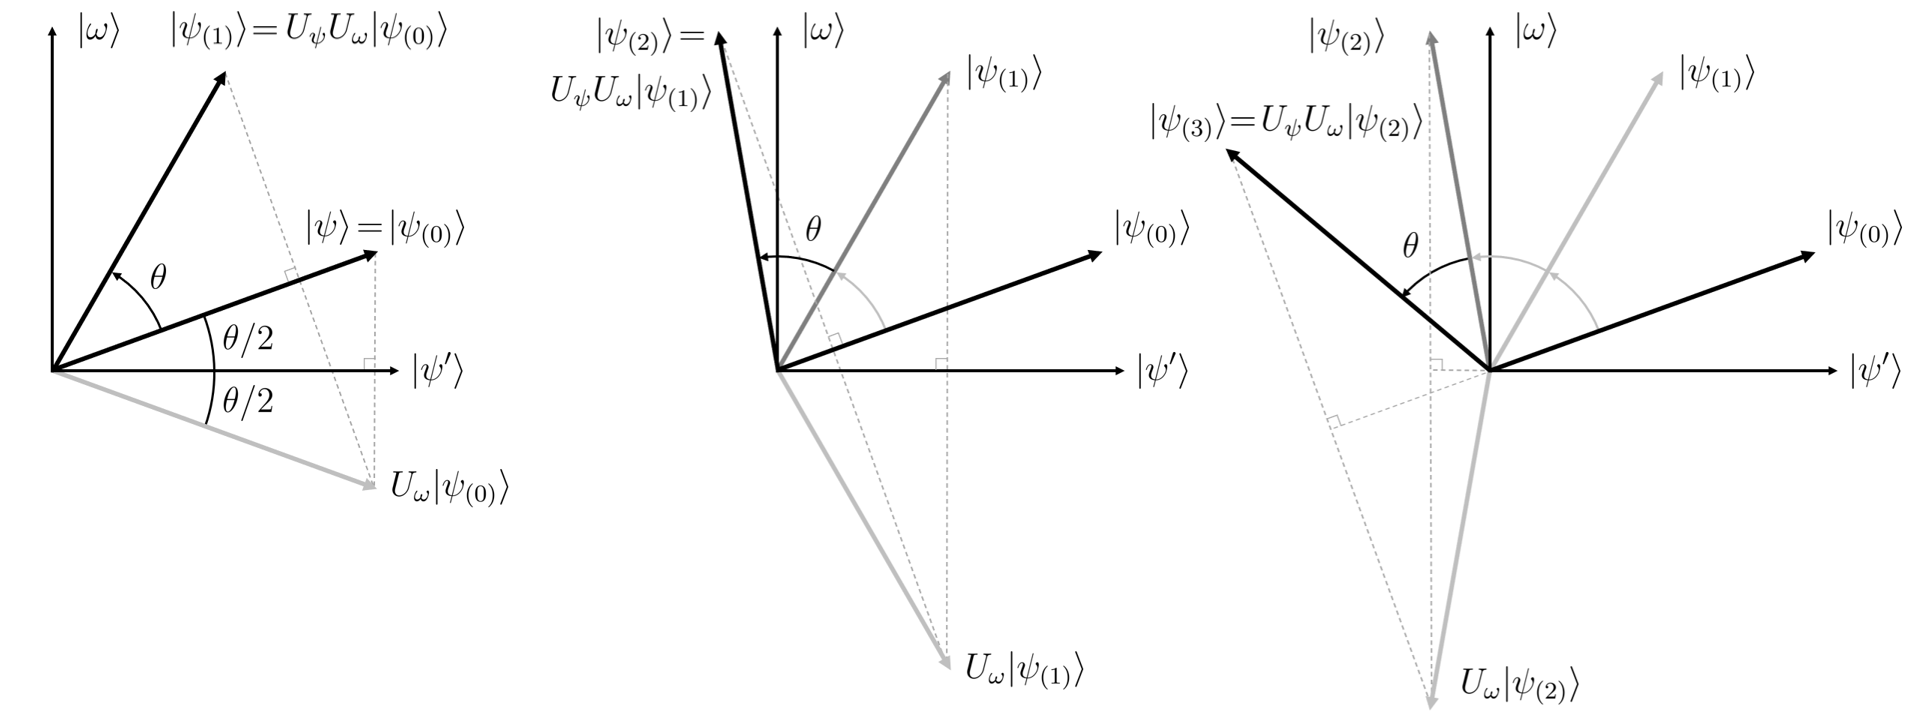
\includegraphics[scale=0.3]{GroverGeom.png}
\end{adjustbox}
\caption{Geometric interpretation of Grover's algorithm}
\label{fig:grover}
\end{figure}
